% Include after all 40 corrected pairs and their generated report are reviewed.
\begin{figure}[p]
\centering
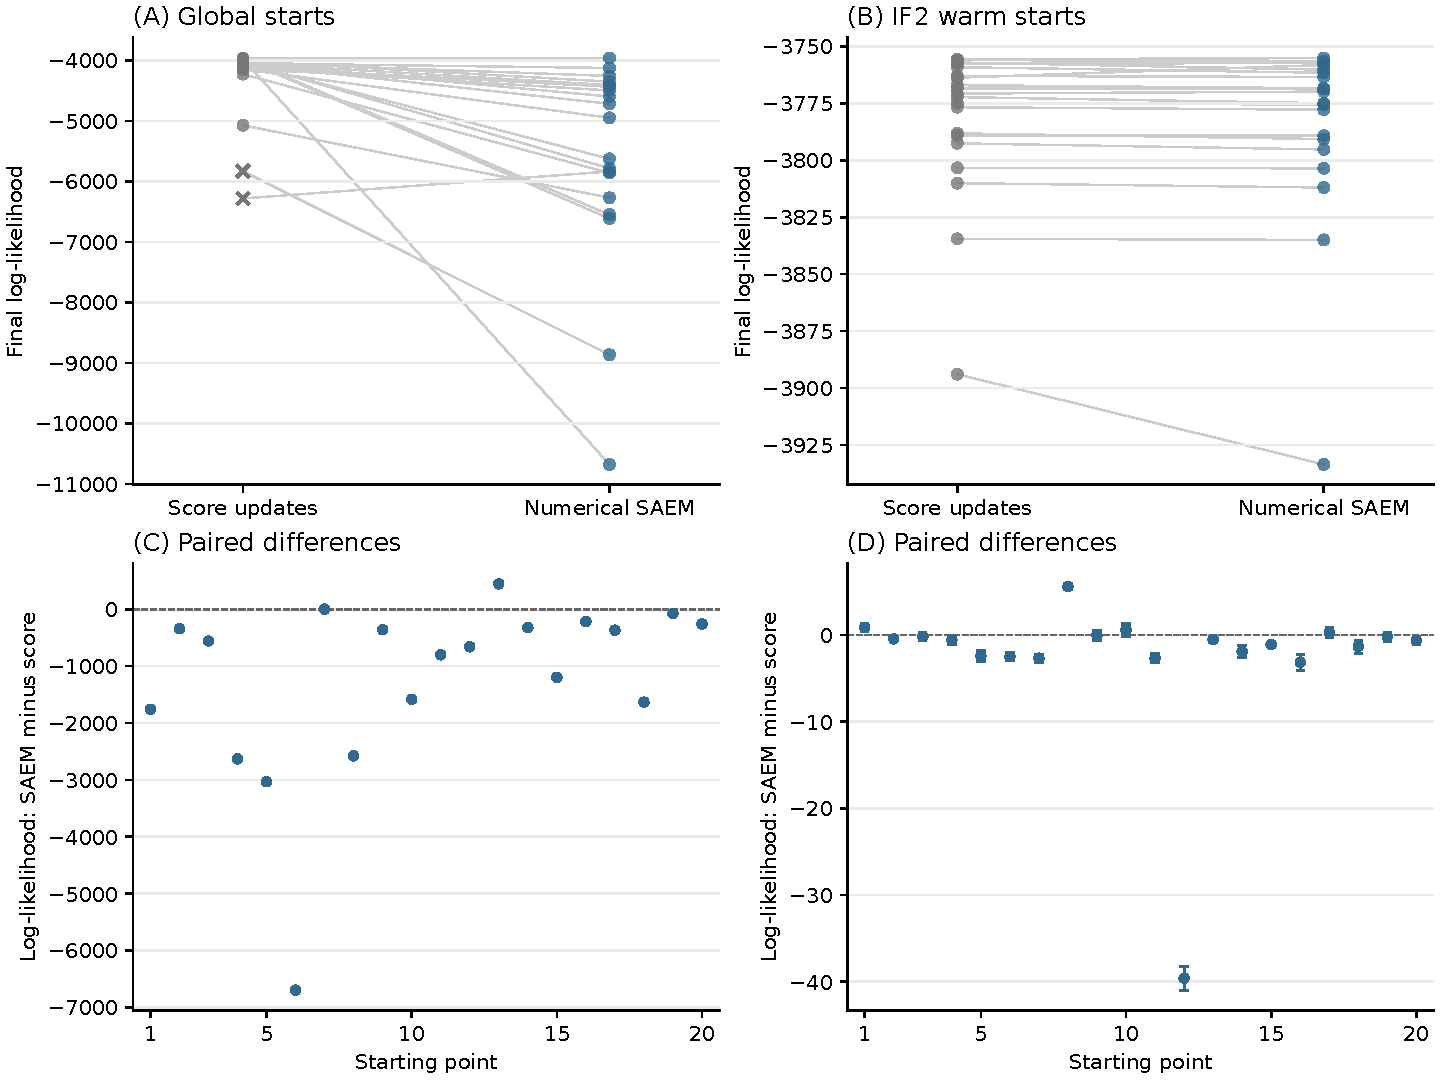
\includegraphics[width=\textwidth]{ditlevsen/results/saem_ab_scaled/report/comparison.pdf}
\caption{Averaged-score updates and numerical SAEM on Dhaka, using the
same monthly Gaussian transition approximation and particle smoother.
Both methods use 1,000 particles and receive 850 seconds per fit, from
20 global starts (A, C) and 20 saved IF2 estimates (B, D).
Panels A and B join final estimates from the same starting point.
Crosses mark prematurely stopped fits, retaining the last eligible estimate.
Panels C and D show paired log-likelihood differences, numerical SAEM minus
score updates; bars show twice the paired Monte Carlo standard error.
Final likelihoods use the original Euler model, with 5,000 particles and
36 evaluation replicates. Evaluation random numbers are shared within a
pair and independent of fitting. All axes are linear.}
\label{fig:dhaka-saem-ab}
\end{figure}

\begin{table}[p]
\centering
{\small
\setlength{\tabcolsep}{4pt}
\begin{tabular}{llrrrrr}
\toprule
Initialization & Optimizer & Median $\ell$ & Median change & Iterations & Time (s) & Failed \\
\midrule
Global & Score updates & -4050.49 & 3827.36 & 86 & 854.5 & 2 \\
Global & Numerical SAEM & -4834.43 & 3109.60 & 15.5 & 851.3 & 0 \\
IF2 & Score updates & -3771.54 & -0.27 & 89 & 855.7 & 0 \\
IF2 & Numerical SAEM & -3772.44 & -1.37 & 13 & 851.1 & 0 \\
\bottomrule
\end{tabular}

}
\caption{Dhaka score and numerical-SAEM comparison in
Figure~\ref{fig:dhaka-saem-ab}.
Median $\ell$ is the median final Euler log-likelihood.
Median change subtracts each fit's initial log-likelihood before taking
the median. Iterations is the median count of completed outer iterations
at the selected estimate, including iterations without a parameter change.
Time is the median duration of the fitting call, including the work needed
to detect a time-limit overrun; over-budget estimates are discarded.
Compilation, independent evaluation and the cost of producing the saved
IF2 starting estimates are excluded.
Failed fits retain their last eligible estimates in all summaries.}
\label{tab:dhaka-saem-ab}
\end{table}
